%%%%%%%%%%%%%%%%%%%%%%%%%%%%%%%%%%%%%%%%%%%%%%%%%%%%%%%%%%%%%%%%%%%%%
% PREAMBLE
%%%%%%%%%%%%%%%%%%%%%%%%%%%%%%%%%%%%%%%%%%%%%%%%%%%%%%%%%%%%%%%%%%%%%
%
% The following two commands will generate a PDF that follows all the requirements for submission
% and peer review.  Uncomment these commands to generate this output (and comment out the two lines below.)
%
% DOUBLE SPACE VERSION FOR SUBMISSION TO THE AMS
\documentclass[12pt]{article}
\usepackage{ametsoc}
\linenumbers
%
% The following two commands will generate a single space, double column paper that closely
% matches an AMS journal page.  Uncomment these commands to generate this output (and comment
% out the two lines above. FOR AUTHOR USE ONLY. PAPERS SUBMITTED IN THIS FORMAT WILL BE RETURNED
% TO THE AUTHOR for submission with the correct formatting.
%
% TWO COLUMN JOURNAL PAGE LAYOUT FOR AUTHOR USE ONLY
%%%%\documentclass[10pt]{article}
%%%%\usepackage{ametsoc2col}
%
%%%%%%%%%%%%%%%%%%%%%%%%%%%%%%%%%%%%%%%%%%%%%%%%%%%%%%%%%%%%%%%%%%%%%
% ABSTRACT
%
% Enter your Abstract here
%%%%%%%%%%%%%%%%%%%%%%%%%%%%%%%%%%%%%%%%%%%%%%%%%%%%%%%%%%%%%%%%%%%%%

\newcommand{\myabstract}{The ADCIRC Surge Guidance System (ASGS) is 
a real time software system for coastal ocean modeling that uses the 
ADCIRC coastal circulation model with optional coupling to the SWAN 
wave model. It is the first generally available real time coastal 
modeling system that is relocatable as well as portable across 
computing platforms. The system was designed with reliability, 
portability, and flexibility as key requirements, and has been 
applied successfully during hurricanes including Irene, Isaac, and 
Sandy as well as the 2010 Deepwater Horizon event. Furthermore, all 
the components of the system are open source and available for 
inspection, collaborative development and widespread independent 
application. The structure, function, and performance of the system 
are described herein.}

%
\begin{document}
%
%%%%%%%%%%%%%%%%%%%%%%%%%%%%%%%%%%%%%%%%%%%%%%%%%%%%%%%%%%%%%%%%%%%%%
% TITLE
%
% Enter your TITLE here
%%%%%%%%%%%%%%%%%%%%%%%%%%%%%%%%%%%%%%%%%%%%%%%%%%%%%%%%%%%%%%%%%%%%%
\title{\textbf{\large{The ADCIRC Surge Guidance System}}}
%
% Author names, with corresponding author information. 
% [Update and move the \thanks{...} block as appropriate.]
%
\author{\textsc{Jason Fleming,}
				\thanks{\textit{Corresponding author address:} 
				Jason Fleming, Seahorse Coastal Consulting, 
				3103 Mandy Ln. Suite 3, Morehead City, NC 28557. 
				\newline{E-mail: jason.fleming@seahorsecoastal.com}}\quad\textsc{and Janelle Reynolds-Fleming}\\
\textit{\footnotesize{Seahorse Coastal Consulting, Morehead City, North Carolina}}
\and 
\centerline{\textsc{Man E. Others}}\\% Add additional authors, different insitution
\centerline{\textit{\footnotesize{Affiliation, City, State/Province, Country}}}
}
%
% Formatting done here...Authors should skip over this.  See above for abstract.
\ifthenelse{\boolean{dc}}
{
\twocolumn[
\begin{@twocolumnfalse}
\amstitle

% Start Abstract (Enter your Abstract above.  Do not enter any text here)
\begin{center}
\begin{minipage}{13.0cm}
\begin{abstract}
	\myabstract
	\newline
	\begin{center}
		\rule{38mm}{0.2mm}
	\end{center}
\end{abstract}
\end{minipage}
\end{center}
\end{@twocolumnfalse}
]
}
{
\amstitle
\begin{abstract}
\myabstract
\end{abstract}
\newpage
}
%%%%%%%%%%%%%%%%%%%%%%%%%%%%%%%%%%%%%%%%%%%%%%%%%%%%%%%%%%%%%%%%%%%%%
% MAIN BODY OF PAPER
%%%%%%%%%%%%%%%%%%%%%%%%%%%%%%%%%%%%%%%%%%%%%%%%%%%%%%%%%%%%%%%%%%%%%

\section{Introduction}

Techniques have been under development since at least the 1950’s to 
quantitatively predict the likely storm surge levels resulting from 
tropical cyclones (Massey et al, 2007). While initial investigations 
were motivated by scientific curiosity, applied studies were later 
commissioned by federal agencies such as the US Army Corps of 
Engineers for storm surge protection designs and by the Federal 
Emergency Management Agency (FEMA) for the purpose of quantifying 
risk and disaster planning. (\cite{LynchDR2004})(\cite 
{ASGSOperatorsGuide2011}) (\cite{ASGSDevelopersGuide2011}) (\cite 
{BlainCA1998}) (\cite{BlainCA2002}) (\cite{BlainCA2002}) (\cite 
{DietrichJC2012}) (\cite{FlatherRA1994}) (\cite{GraberHC2006}) (\cite
{HollandGJ1980}) (\cite{HoustonSH1999}) (\cite{HubbertGD1991}) (
\cite {LynchDR2004}) (\cite{MasseyWG2007}) (\cite{OConnorWP1999}) (
\cite {VerlaanM2005}) (\cite{XieL2006}) (\cite{MattocksC2006}) (\cite
{RamakrishnanL2006})(\cite{KennedyA2010})(\cite{FlemingJG2008}) (
\cite{GlahnB2009})(\cite{GlahnB2009}) (\cite{KimSC1996})(\cite
{BlainCA2002Tidal})(\cite{BlantonBO2012}) (\cite{VanCootenS2011})(
\cite{BooijN1999})(\cite{ChuP2009})

Over the course of time, the approach to numerical storm surge 
calculations evolved in two separate directions: simulations that 
were meant to be used operationally, and those that were meant to be 
used in an offline design study. Although both approaches relied 
heavily on probabilistic formulation of the input and statistical 
interpretation of the output, the availablility of computational 
resources that could be applied in each case was assumed to be 
different. The model implementations meant for operations were 
required to run with lower resolution and lower provision of 
computational resources than model implementations used for offline 
design studies. 

This bifucation of approach to resource requirements was strongly 
evident during the approach and landfall of hurricane Katrina on the 
northern Gulf coast of the US in 2005. The storm surge forecasts 
that were produced in real time for Katrina contained far less 
detail and realism than the coastal engineering design studies that 
were commonly performed at that time using ADCIRC. 

As a result, in the aftermath of Katrina, there was strong 
motivation to bring the detail, realism and computational resources 
of a design study to bear in real time.  

As the technology supporting numerical storm surge calculations 
developed over time, the value of the predictions for real time 
emergency response became more and more clear (\cite 
{JelesnianskiCP1992}). The first attempt to apply an existing 
coastal model in a real time context was the SLOSH model (\cite 
{JelesnianskiCP1992}). This system was developed according to the 
``closed system'' paradigm depicted in Figure 1. In this approach, a 
small unified team of developers within a single organization takes 
responsibility for every aspect of the system: gathering of physical 
(e.g., bathymetry), construction of a meteorological model, offline 
validation, computational resources, post processing, visualization, 
dissemination to end users within the same organization, and the 
software automation to make the whole stack run in real time. 

The advantages of the closed system approach are simplicity and 
control. Simplicity results from the need to only code for a single 
computational plaform with a narrow set of capabilites as required 
to satisfy the target audience. All other things being equal, simple 
systems are more reliable and easier to maintain than complex 
systems. Closed systems are also easier to control. This ease of 
control stems from the availability of dedicated resources, 
including compute time, staff time, and a single chain of command 
with high level buy-in for the stated objectives of the real time 
guidance system.

The disadvantages of the closed system are expense, inflexibility, 
and stagnation. Closed systems are relatively expensive because all 
research, development and maintenance costs must be borne by a 
single working group within an organization. New features and 
capabilities can only be produced as the time and budget of that 
group allows, and development of new capabilities must be balanced 
against the need to maintain and operate.

Because closed systems are developed for a narrow target audience on 
a single target platform, many simplfying assumptions may be made to 
speed development, thus reducing the initial cost. But these 
simplifying assumptions also serve to stymie later extensions to new 
compute platforms, new geographical areas, or the inclusion of new 
features. 

The final disadvantage of closed systems is stagnation. The lack of 
technology sharing with other working groups, or applications for 
other projects or end users tends to limit the expansion of the 
technology to new areas, especially those outside the experience of 
the foundational team. 

An alternate architecture that we call the ``distributed chain'' is 
illustrated in Figure 2. This type of system is the polar opposite 
of the closed system described previously. The distributed chain 
system distributes the load and responsibility of developing each 
piece of a real time guidance system to several geographically 
dispersed organizations that are linked through the internet via a 
common data bus that is used to download products, then upload them 
after some processing or contribution to the final result. For 
example, one organization may be run a numerical weather model, 
while another orgainzation sets up a surge model, with computational 
resources being offered by yet another organization. 

The advantages and disadvantages of the distributed chain system are 
mostly the inverse of the closed system. The disadvantages are 
complexity and lack of control: each time another institution or 
software system are included in the chain, the system becomes more 
complex and the number of potential points of failure increases. The 
increase in the number of failure points is particularly significant 
because the chain is only as strong as its weakest link. And because 
each link in the chain is operated independently, there isn't a 
single point of accountability for all of the participants.

The advantages of the distributed chain are flexibility and 
vibrancy. Because of the open-participation philosophy and sharing 
of a common data bus, the barrier to entry of new participants and 
new ideas is low, and as a result such architectures attract new 
ideas and new participants easily.

On the issue of expense, it is difficult to determine whether the 
closed system or the distributed chain have the advantage. The 
distributed chain distributes the cost of development among several 
participating teams, so the expense associated with any given team 
is lower. However, the aggregate cost of the whole distributed chain 
may not be lower, as it includes the increased costs associated with 
coordinating the various participants. 

Finally both closed systems and distributed chains face the burden 
of reinventing the wheel when implemnting new features, and even 
issues of long term viability; these issues result from a lack of 
freely shared technology. Closed system technologies and the 
individual components of distributed chain systems are generally 
kept ``in-house'' and not freely shared with other developers 
outside the organization. As a result, technological features must 
be created from scratch whenever a new group decides to develop a 
real time coastal forecast system. Furthermore, the products of 
these teams will continue to be available only from their original 
developers and only for as long as they are able to produce them, 
and the issues of stagnation still apply to those technologies.

In order to combine the advantages of both the closed system and 
distributed chain approaches while avoiding their respective 
disadvantages, the ASGS has been developed using a regional team 
approach. In this paradigm, shown in Figure 3, the technology and 
know-how associated with it are freely shared among participants, 
while the responsibility for local validation, securing computational 
resources, real time execution and communication with local emergency
manager and high level officials are distributed to regional teams 
to apply the ASGS to issues of local interest. 

The regional team approach offers the flexibility and vibrancy of 
the distributed chain, since the existing technology is freely 
shared among participants, enabling new participants to get up to 
speed quickly while existing participants benefit from sharing  new 
features. It also solves the weakest link and accoutability issues 
inherent in the distributed chain approach, since each regional team 
operates independently in a self-contained way during a real time 
event, and each team is subject to a single local chain of command and 
coordination in real time.

The expense of the regional team approach is relatively low, 
particularly for new participants, because the burden of ongoing 
maintenance efforts and new feature development is distributed among 
all participants, while the benefits of those efforts are shared by 
all, preventing any regional team from having to reinvent the wheel. 
However, in order for the benefits of technology sharing to accrue, 
a central coordinator or guide must take responsibility for 
integrating disparate features, developing new features in the 
underlying numerical model(s) to support new capabilities in the 
software automation system, writing or aggregating documentation, 
ensuring continuity, and providing training or capacity building. 

Finally, and perhaps most importantly, securing computational 
resources with the regional team approach is cheaper and easier than 
through any other approach. Regional computing centers have an 
inherent incentive to provide resources to support real time 
modeling for a current event that is directly relevant to their 
local environment, and a disincentive to provide resources for 
events that are not locally relevant. This dovetailing of interests 
greatly simplifies and facilitates access to computational 
resources, and in our experience this advantage should not be 
underestimated. 

\subsection{Challenges}

The provision of any sort of real-time prediction of storm surge is 
challenging for many reasons, including (1) uncertainty in the storm 
forecast (which translates directly into uncertainty in the 
predicted surge; (2) an extremely short shelflife of results (i.e., 
model results may go from lifesaving to useless in a matter of 
hours; and (3) storm surge results are sensitive to wind forcing but 
high quality wind data are not available until several hours after 
the corresponding forecast advisory has been issued. 

In addition, there are particular challenges associated with the 
offsite production of storm surge predictions in a real time context 
from a general-purpose coastal circulation model such as ADCIRC, 
including the following: (1) ADCIRC is capable of producing results 
at high resolution but requires supercomputer-level computational 
power to do so; (2) the input wind data from an offsite source is 
voluminous and requires high-bandwidth connections for transmittal 
in a reasonable pe- riod of time; (3) the on-demand availability and 
99.999\% reliability requirements for real time storm surge 
forecasting system are far higher than are normally required of a 
shared-use super- computer and commercial grade internet 
connections; (4) redundancy may be employed to increase reliability 
and availability of results but also increases complexity as well as 
requiring portability; (5) the results must be post-processed and 
reliably delivered to off-site end users in a form that is useful 
while communicating the underlying uncertainty and without causing 
confusion. 

The following sections describe how a generalized real time storm 
surge forecasting system was developed to meet each of the 
challenges outlined above. The application of the system to a case 
study site is then described, and conclusions about the systems 
performance are provided.

\section{Methods}

In this section, each of the methods used to meet the the previously 
described challenges is provided. A detailed description of the 
method for arriving at the meteorological forcing based on the 
forecast advisory from the National Hurricane Center is provided. 
The methods used to provide results in a timely manner are discussed 
in principle and then a detailed description is provided to show the 
methods in practice. Finally, the measures taken to assure the 
reliablility of a real time storm surge forecast system based on 
a generalized coastal ocean model are discussed.

\subsection{Overview}

A brief description of how the ASGS conceptualizes the operation of 
ADCIRC or ADCIRC+SWAN into three phases: hindcast, nowcast, and 
forecast. 

Then describe what happens in each phase: the hindcast is for 
spinning up tides and/or initializing rivers while meteorological 
forcing is turned off. 

The nowcast is for updating the current state of the simulation from 
where it left off at the end of its last execution (could be either 
a nowcast or hindcast) to the start of the current set of forecast 
data. The nowcast uses data that are considered definitive over the 
time period being covered, that is, not speculative forecast data. 
Parameter variations are not allowed during a nowcast. 

The forecast is speculative, meaning that the input is a representation
of a possible future state, and a wide variety of parameter variations
are enabled for constructing an ensemble of forecasts to cover the possible
range of future states, or to construct ``what-if'' scenarios.

\subsection{ADCIRC}

Brief boilerplate description of the ADCIRC model.

\subsection{SWAN}

Brief boilerplate description of the SWAN model.

\subsection{ASGS Structure}

An overview of the modular structure of the ASGS is shown in Figure 
1. The figure indicates the separation of components into (1) 
reference information (in purple), which specify the system 
configuration and physical parameter data used in the simulation; 
(2) dynamic input data (in red) that varies in time and must be 
downloaded from external data sources for every forecast cycle; (3) 
input file production (in green), which implements the system 
behavior specified by the user in the system configuration files; 
and (4) output visualization, publication, and interaction (in blue) 
for use by clients and end users. These modules will be described in 
greater detail below. 

\subsection{Reference Data}

The reference information includes a dynamic specification of system 
behavior in the configuration file as well as static physical data, 
embodied in the simulation input files ADCIRC. The system 
configuration consists of a single file, and all of the features and 
behavior of the various components can be controlled from this 
single configuration file. This file is used to activate or 
deactivate the various types of physical forcing, including tropical 
cyclone meteorology, ordinary meteorology, wave simulation and 
coupling, tides, and river flow input. It is also used to specify a 
wide variety of other settings, including (for example) the type of 
computer that the system is running on, the number of processors to 
use in parallel execution, the name of the ADCIRC mesh file for the 
domain of interest, the number of storms in an ensemble and their 
characteristics, the types of output products to generate, the email 
addresses of officials that should be notified when results are 
ready, and many others. 

The simulation input files represent a purely static set of physical 
data that are used in the simulations. These data include the ADCIRC 
mesh (domain discretization), the bathymetry and topography of the 
domain, the spatially varying Manning's n value, and the directional 
wind roughness lengths and canopy effects derived from land cover 
data. The static data also include the tidal constituents to be 
included (if any), convergence controls and solution parameters for 
SWAN and ADCIRC, the names and locations of point recording stations 
for location-specific output data, and other data related to the 
internal procedures of the simulation codes. 

\subsection{Dynamic Input Data}

The application of meteorological forcing presents a challenge for 
real time storm surge forecasts because of the need for timely 
availability of input data as well as additional preprocessing 
delays associated with large meteorological datasets. The most 
accurate data-assimilated meteorological fields are not available 
until several hours have passed after a corresponding hurricane 
advisory from the NHC. When they do become available, a 
preprocessing step must be performed to interpolate the data onto 
the storm surge grid, which may introduce significant delays for 
very large input datasets. 

Other disadvantages include the fact that 
they have a relatively coarse resolution in comparison to the 
underlying simulation grid, and the fact that they may include 
meteorological information far from the area of interest. In 
contrast, parametric wind models produce comparable storm surge in 
many cases (Houston et al, 1999; Mattocks et al 2006). They also 
have the advantages that they require a comparatively tiny quantity 
of input data and that they may be coded as fast subroutines that 
run in-process and can provide wind stress and barometric pressure 
values at arbitrary locations. As a result of the advantages that 
parametric wind models have for the present application, the Holland 
model (Holland, 1980) was selected as the basis of the wind speed 
and pressure field. Modifications and additions were made to the 
published model to account for the dynamic changes in the hurricane 
parameters along the hurricane’s track, as well as its adaptation to 
the data available from the NHC advisory. This modified model will 
be referred to as the Dynamic Holland model.

\subsubsection{North American Mesoscale Model}

The system is capable of downloading and preparing dynamic 
meteorological data from two sources: the National Hurricane 
Center's (NHC) Forecast/Advisories, and the National Centers for 
Environmental Prediction's (NCEP) North American Mesoscale (NAM) 
model, depending on the data source selected by the Operator. 
Furthermore, the system has a module for downloading river boundary 
flow data from the National Severe Storms Laboratory and preparing 
it for use in ADCIRC.

\subsubsection{Asymmetric Vortex Model}

For tropical cyclone events, the NHC Forecast/Advisories are 
downloaded by the system as soon as they are issued, and the 
relevant storm parameters (including storm positions. maximum wind 
speeds, and isotach radii) are parsed into a format that ADCIRC can 
use to generate wind fields using an internal asymmetric vortex 
model. For ordinary meteorology, including nor'easters and other 
systems, the system downloads regularly gridded meteorological 
fields from the NAM model from the NCEP ftp site. The gridded 
meteorological fields are extracted from the grib2 format that NCEP 
uses, reformatted and written to OWI formatted files that ADCIRC 
reads. 

\subsubsection{River Flux Forcing}

Once meteorological data have been obtained, the system downloads 
the latest river flow data from the National Severe Storms 
Laboratory (NSSL) ftp site. These data are in a file format that 
ADCIRC can read natively, and are set up to correspond to a 
particular ADCIRC mesh. The module that downloads these data must 
splice a series of these files together to match the date and time 
range implied by the meteorological data that have already been 
obtained. 

\subsection{Input File Production}

Once the Operator has created a configuration file and assembled the 
static physical input data for a particular instance of the system 
and initiates startup, the system reads its configuration file and 
tries to determine its state: whether it is starting “hot” with a 
simulation that is already in progress, or “cold”, where a new 
ADCIRC or ADCIRC+SWAN simulation must be started from scratch (see 
Figure 2). It also makes a determination about the state of its 
input files; specifically, whether they have already been decomposed 
for parallel execution. If the system must start from a “cold” 
state, it creates input files and executes a hindcast simulation to 
warm up the simulation and prepare it for the cyclical 
nowcast/forecast production phase (described below). Accordingly, 
this hindcast run is set so that it writes a hotstart file at the 
very end to represent the state of the warmed-up simulation. In 
addition, if the input files have not been prepared for parallel 
execution, the system decomposes them for the specified number of 
processors. If the hindcast and/or decomposition tasks are required, 
they must only be performed once at the start of the system's 
execution (processes that occur at most one time during an execution 
of the system are shown in blue in figure 2).

The nowcast occurs next if the simulation state is already "hot" 
when the system starts up, or if the system has already performed 
the decomposition and warm up phases. The first step in the nowcast 
is to determine if there are new meterological data available, by 
contacting the associated external website or ftp site, checking the 
timestamps that are available there, and comparing them with the 
current simulation time. If there are data available that are more 
recent than the current simulation time, a new cycle is deemed to 
have begun, and those data are downloaded. The system downloads the 
data it requires to cover the time period between its current 
simulation time and the most recent data that are available files 
that are available. After the meteorological data have been 
acquired, river data are acquired in the same way, if they have been 
specified. 

Once the external data have been acquired, the input files for the 
ADCIRC simulation code (and the SWAN simulation code if wave forcing 
has been specified by the Operator in the system configuration file) 
are constructed using the time range of the meteorological forcing 
files and the various configuration parameters in the system 
configuration file. This includes tidal boundary conditions, output 
file formats and frequency of production of output files, and 
locations for point recording of output for comparison with tide 
gages or meteorological data collection equipment. The nowcast 
control file(s) for ADCIRC and SWAN are set to write a hotstart file 
at the end of the simulation for use in starting the forecast, as 
well as a future nowcast. The last file written during the nowcast 
phase is the queue script that will be used to submit the job to the 
high performance computer's queueing system.

Once the nowcast is complete, the system acquires the data required 
for one or more forecasts. These data will already be present in the 
case of a tropical cyclone, since the NHC forecast/advisory has 
already been parsed. For NAM forcing, the NAM forecast data are 
downloaded from NCEP and converted to OWI using the same technique 
as described for the nowcast. If river flux forcing was specified, 
the river flux data are downloaded and formatted in a similar manner 
to the nowcast. The control files are constructed to cover the time 
period implied by the forecast meteorological data, but are not set 
to write a hotstart file at the end. When the forecast is complete, 
the system executes post processing (described in the next section) 
and archives the data as required. 

These forecast process described above is applied to  each member of 
the forecast ensemble until all ensemble members have been 
completed, at which point the system goes back to looking for new 
meteorological data for its next nowcast.

\subsection{Flexibility}

Definition of what we mean by flexible: different types of forcing 
can be configured, configuration is centralized so that different 
capabilities can be meteorological models are possible. Flexibility 
also comes from the use of standards, including dissemination 
standards such as OpenDAP as well as metadata standards. This 
flexibility allows the use of multiple different types of post 
processing including built in (non-interactive) post processing like 
FigureGen, RenciGETools as well as interactive post processing like 
CERA and AdcircViz.

\subsection{Reliability}

Reliability in operation is mostly the result of the self-contained 
nature of the system, which avoids the weakest link and on-call 
issues associated with the distributed chain architecture. It also 
results from having many checks, fail-safes, and retries built into 
the various modules of the system that address and work around issues
that arise during real time operation. 

\subsection{Extensibility}

Extensibility stems from the ability to plug in new capabilities
either in a forecast ensemble or in 

\subsection{Maintainability}

A system that has developed over time without a focus on 
maintainability will gradually lose flexibility and become more and 
more difficult to fix and upgrade. 

Maintainability comes from several factors, the most important of 
which is the use of computer languages that are widely used and well 
understood in the coastal modeling community, such as shell 
scripting and Fortran (and to a lesser extent, perl) while avoiding 
languages that may be more capable but have a much smaller user base 
in the coastal modeling community (such as Java).  

Documentation is critical to maintainability of a shared software 
automation system to prevent a loss of continuity during inevitable 
staff turnover.

\subsection{Affordability}

Development that allows local teams to solve the issues that are 
within their core competencies while receiving the benefit of the 
knowledge and capabilities of other participants allows the fastest
progress of all participants at the lowest cost for each of them.

\subsection{Availability}

In contrast to closed systems, the long term viability of a widely
available system is never in question.  

\subsection{Coordination}

As in any project with a distributed workload and multiple 
objectives, a certain level of central coordination or point of 
contact is necessary to prevent splintering and provide guidance for 
integration of new features, fixes, and new lines of development. In 
addition, some new features of the software automation system
may require new developements in the underlying software, and that these
developments be coordinated. As a result, the development and maintenance
process benefits from the participation of a central development 
coordinator. 

In the context of operation, whether in a real time event such as 
the approach of a tropical cyclone, or in the provision of 
day-to-day guidance, the self-contained and independent nature of 
the operation of the ASGS means that local coordination is all that is
necessary to ensure that the system operates as expected. 

\subsection{Portability}

How the goal of portability was achieved in the ASGS. It starts with 
the portability of the underlying numerical models. Portability is achieved
via: the init subroutines in the shell script, plus case switch statement for
the queueing system in asgs main.sh, a custom template for submitting 
jobs, and possibly a custom template filler script. 

\subsection{Relocatability}

Relocatability basically rests on the system not making any assumptions 
about the underlying mesh. In its current incarnation, the Operator must
supply the mesh and an adcirc control file that contains any static 
boundary conditions (for example, the amplitude and phase of tidal 
constituents along the boundary). 

\subsection{Forecast Ensemble}

A brief description of how an ensemble of storms is configured, 
and the types of variations that are possible. 

\subsection{Output Visualization, Publication, and Interaction}

The production of human-comprehensible output is arguably the most 
important step in the entire process. Clients must be notified that 
new results are available; and they must be able to get to and use 
the results in a way that is  intuitive for them. As there is more 
than type of end user or client, there is more than one approach to 
producing useful output: (a) publication of raw data; (b) production 
and publication of static images, non-interactive animations, and 
results files in domain specific formats; and (c) elucidation via 
interactive visualization through a web application.

Publication of raw results is the most basic step for post 
processing, and an OpenDAP server was selected and used to publish 
raw data in NetCDF format to clients and end users. An OpenDAP 
server provides a web interface to the data, making it easy for 
users to simply click on a link to the graphics or data file they 
wish to download, either for the latest run or for any previous 
simulation run.  Technologies such as NCTOOLBOX are available for 
sophisticated end users to apply their own analyses to the raw data, 
producing the output they require locally.  Once the data have been 
posted to the OpenDAP server, the system sends an email to a list of 
email addresses as specified in the system configuration file to 
notify them that new results are available. 

The next level of presentation is in-situ post processing, that is, 
running non-interactive graphics generation programs in the high 
performance computing environment to generate static images, 
non-interactive animations, and reformatted versions of results in 
specialty fomats. These techniques are all in currently place, and 
have the advantage of not requiring voluminous quantities of data to 
be moved to an external server for post processing. For example, the 
system produces GIS shape files, JPEG images and non-interactive 
animations of maximum inundation as well as Google Earth (kmz) 
images of maximum inundation, all with in-situ post processing. 
These output products are then published to the OpenDAP server to 
make them available to clients. The disadvantage of in-situ 
processing is the lack of interactivity. 

The highest and by far the most effective level of presentation is 
the use of an interactive web visualization application to elucidate 
results. For this level, the Coastal Emergency Risks Assessment 
(CERA) interactive web application was deployed and used to provide 
an interactive interface that served the needs of non-technical as 
well as experienced clients. 

The CERA application integrates visualization ADCIRC and ADCIRC+SWAN 
results with Google Maps to provide the context for the results as 
well as practical features such as panning and the ability to zoom 
in more closely at various areas of interest to see greater 
resolution and detail. The application organizes results by storm 
and advisory (for tropical cyclone results) or by cycle (for NCEP 
NAM results). It presents these options concisely via dropdown boxes 
across the top of its interface.

The right side of the interface is an accordion-type menu that 
presents the various types of data that are available, including 
water surface elevation, inundation, significant wave height, wave 
period, and wind speed. For each type of data, the application is 
able to present a zoomable image of the maximum values that occurred 
over the course of the forecast (e.g., high water marks) as well as 
a zoomable, stoppable animation that illustrates the evolution of 
the data through time. 

Furthermore, the interface allowed the user to click on any point of 
the storm track to view the data that are relevant to the time when 
the storm was at that point in the track. It is also capable of 
presenting the nodes of the underlying ADCIRC mesh, and displaying 
detailed summary information for any particular node the user 
selects. 

The CERA application works by using the OpenDAP server as a staging 
area for raw data. The CERA application received notification email 
from the NCFS that new results were published to the OpenDAP server 
in NetCDF format. It would then download these data as well as some 
summary information about the type of forecast run that produced the 
data. It generated visualizations via production of image tiles at 
progressively finer scales, thus providing the user with the ability 
to zoom in and examine results in greater detail. These image tiles 
were then stored on the web server where the data were published, 
and sent to web clients as required by the user interaction with the 
web application and its menu system.

\subsection{Reliability}

Speed and accuracy are useless if the results cannot be produced 
because of software or hardware issues. The most important causes of 
reliability problems includes bugs in the forecast system code, 
hardware failures, unexpected changes in the underlying software 
environment, insufficient availability of shared computer resources 
(usually CPUs), changes in forecast data format or provi- sion, 
numerical instability, failures of webserver machines where results 
are published, and network communication failures. In order to limit 
exposure to risk from many of these issues, the system was designed 
to be self- contained on a single supercomputer, as opposed to 
distributing simulations across several machines, or running 
simulations on one machine and performing post processing on 
another, for example. The computer that the system is running on 
will download the hindcast and forecast, preprocess the input, 
submit all jobs, check for their completion, post process results 
(including drawing the graphs), and then communicate the results to 
end users and system operators. Communication starts with an email 
to the operators to notify them that a new advisory has been 
detected. When the simulations have finished and post processed, the 
resulting graphs are transmitted to a designated webserver (or 
servers) and then another email is sent out to operators and end 
users with representative graphics attached. That email also 
contains a hyperlink to the full results on the webserver. Because 
the entire system is self-contained on a single machine, redundancy 
can be used to further enhance reliablity by simply installing and 
running the system on additional machines, where it will operate 
independently. The redundancy concept may also be applied to the 
communication of results by configuring additional webservers to 
receive results as they are produced. The least often encountered 
reliability problems are in the data source and the model itself. 
The data source (the NHC) rarely makes changes, and adjustments are 
easy to make. Preventing numerical instabilities is mostly a matter 
of good grid design. If a numerical instability issue were to occur, 
it would not create a real problem unless it occurred during a 
nowcast run, since errors in forecasts do not propagate to the next 
advisory cycle.

\subsection{ADCIRC Asymmetric Vortex Model}

The application of meteorological forcing presented a challenge for 
real time storm surge forecasts because of the need for timely 
availability of high resolution input data. The most accurate 
data-assimilated meteorological fields from the H*Wind project were 
only available for nowcast and hindcast times, and even then were 
not available until several hours had passed after a corresponding 
hurricane advisory had been issued from the NHC. In addition, 
regularly gridded meteorological data from models such as the North 
American Mesoscale (NAM) model had a relatively coarse grid 
resolution in comparison to the unstructured ADCIRC mesh (12km grid 
resolution vs 30m minimum mesh resolution).

In contrast, parametric wind models produce comparable storm surge 
in many cases (Houston et al, 1999; Mattocks et al 2006). They also 
had the following advantages: (1) they require a comparatively tiny 
quantity of input data; (2) they could be coded as fast subroutines 
that run in-process; (3) they could provide wind stress and 
barometric pressure at arbitrary locations.

As a result of the advantages of parametric wind models, the Holland 
model (Holland, 1980) was selected as the basis of the wind speed 
and pressure field. Modifications and additions were made to the 
published model to account for the dynamic changes in the hurricane 
parameters along the hurricane's track, as well as its adaptation to 
the data available from the NHC advisory, as described below. This 
modified model was referred to as the Dynamic Asymmetric Holland 
Model.

\subsection{Dynamic Asymmetric Holland Model}

The hurricane advisory contained at least the following information 
for each forecast increment: date, time, latitude and longitude of 
the center of the storm, and maximum observed wind speed at 10m with 
a 1 minute sampling interval. In addition, the distance to isotachs 
at various wind speeds were sometimes provided in one or more storm 
quadrants.

The vortex model was set up to operate in a two step process. The 
first step was the use of isotach data from the forecast/advisory to 
calculate a representative radius to maximum winds (Rmax) in each of 
the four storm quadrants, for each forecast increment, before the 
actual ADCIRC run. The second step was to interpolate the resulting 
Rmax for all nodes at each time step of the simulation, to determine 
the wind velocity throughout the domain at each time step.

The first step was performed in a pre-processing program for all the 
data from a particular forecast/advisory, before the ADCIRC run 
began. This design provided visibility to the Rmax values that 
ADCIRC would use, and gave the user the capability to modify the 
input values for experimentation.

The representative Rmax values were determined for each quadrant and 
forecast increment by subtracting the translation speed of the storm 
from the maximum wind speed, and converting both the 
translation-reduced maximum wind speed and the highest isotach wind 
speed in that quadrant into the equivalent wind speeds at the top of 
the atmospheric boundary layer. These wind speeds and the distance 
to the highest isotach in that quadrant were then substituted into 
the gradient wind equation. The gradient wind equation was then 
solved for the Rmax in that quadrant using Brent's method, or if 
that failed numerically, a brute force marching algorithm.

The pre-processing program then appended the resulting Rmax values 
to the meterological input file for use in the actual ADCIRC 
simulation.

The second step occured during the execution of ADCIRC. For each 
time step in the simulation, the central pressure, latitude and 
longitude of the storm center, and radii to maximum winds were 
interpolated in time to reflect the simulation time relative to the 
forecast increments provided by the National Hurricane Center. The 
translation speed from the most recent forecast increment was used 
to reduce the time-interpolateed maximum wind speed. The 
time-interpolated maximum wind radii were interpolated in space 
using a cubic spline; the relevant value of Rmax at each node was 
determined from the cubic spline curve. Finally, the Holland(1980) 
model was used to determine the nodal wind velocity using the 
spline-interpolated Rmax, the translation-reduced value of the 
maximum wind speed, and a Holland B whose value was calculated and 
then limited to the range of 1.0 to 2.5.

After the computation of the nodal wind velocities at the top of the 
atmospheric boundary layer, the magnitudes were reduced to 
corresponding values at 10m, and then reduced again from the 1 
minute averaging used by the National Hurricane Center to 10 minute 
averaging required by ADCIRC. A "damped" translational velocity was 
vectorially added to the nodal wind velocities, where the damping 
was proportional to the distance from the radius to maximum winds.

Finally, the wind vectors were rotated toward the center of the 
storm by an angle that depended on the distance from the center: the 
rotation angle was ten degrees between the center and the radius to 
maximum winds; it was twenty five degrees beyond 1.2 times the 
radius to maximum winds; and the rotation angle was linearly 
interpolated from the ten degree value at Rmax and the 25 degree 
value at 1.2 times Rmax.

\section{Results}

In order to demonstrate the utility of the generalized forecast 
system, recent applications of the ASGS and their results will be 
highlighted.

\subsection{Deepwater Horizon}

Brief description of how the ASGS was used during Deepwater Horizon in 2010.

\subsection{Irene}

During Hurricane Irene of 2011, the ASGS and CERA technologies were 
actively and heavily utilized by National Weather Service (NWS) 
offices, emergency managers, and the US Coast Guard. In one example 
of the real benefit for emergency management officials, US Coast 
Guard Admirals personally operated the web application to examine 
and interact with simulation results, and then used those results in 
their decision to evacuate their command center near Norfolk, VA, 
relocating to their secondary command center in Missouri. 
Subsequently, the predicted flooding did occur, rendering the 
abandoned USCG command center useless. In summary, the USCG was able 
to maintain uninterrupted command and control over the course of 
Hurricane Irene from their alternate command center, and have lauded 
the ASGS/CERA system for its contribution to this successful 
real time decision.

Hurricane Irene 2011 provided an oppportunity to use the ASGS and 
CERA technologies to assist officials in the NWS and USCG with 
real-life and emergency management decisions in real time. The 
implementation of these technologies for the North Carolina and US 
East Coast that provided the basis for this real life application 
are described below, including the static physical data, use of 
dynamic meteorological and river flow data, configuration, 
interaction with web-based results, and feedback from official end 
users. 

\subsection{North Carolina Physical Data}

The discretization of the North Carolina domain (the mesh) that was 
used for both ADCIRC and SWAN is shown below in figure 3. The mesh 
contained 295328 nodes and 575512 with a minimum element size of 
13m. The land cover data that were used to derive directional wind 
roughness lengths, canopy coefficients, and Manning's n friction 
values are shown in figure 5. The system set 127 points throughout 
the domain for sampling the model output for comparison with tide 
gauges and water levels in river flood plains and other locations. 
It also specified 99 locations for point sampling of model 
meteorological data for comparison with physical meteorological data 
collected at land based and buoy-based meteorological data collected 
by various state and federal agencies and universities.

\subsection{Dynamic Input Data}

As the storm that would eventually become Irene was forming, the 
ASGS/CERA system had already been running for months at RENCI on the 
blueridge machine, a 1408 core Dell High Performance Computing 
cluster, producing daily forecasts using NCEP NAM meteorology, river 
flow data from NSSL, and tidal forcing. 

When Irene formed and the decision was made to start running 
vortex-forced tropical cyclone forecasts, a new instance of the ASGS 
was started up from the most recent hotstart file from the existing 
NAM results. The new instance was configured to run on 384 
processors, rather than the 180 that were used in the NAM runs. Both 
ASGS instances then ran side by side for several days, sending their 
output to the CERA web application, until the NAM instance was shut 
down to conserve processor time.

\subsection{Internally Generated Input Files}

On 384 processors, the ASGS was able to perform all file 
manipulations for the nowcast and forecast cycle for the consensus 
track, submit the jobs, and generate results for a 5 day forecast in 
1 hour 15 minutes from the time the NHC forecast/advisory was issued. 

As hurricane Irene approached the North Carolina coast, the team 
member that operates of the ASGS system lost electric power and 
could therefore no longer oversee the operation of the ASGS during 
this critical period. However, since the ASGS itself was actually 
executing at the RENCI facility, which is located in Durham, North 
Carolina and that facility never lost power, the ASGS was able to 
continue operating autonomously without interruption and without 
interaction or oversight for the duration of the storm.  

\subsection{Output Visualization and Interaction}

The results produced by the ASGS were converted in-situ to Google 
Earth (kmz) graphics and posted to the OpenDAP server at RENCI for 
use by the Newport NWS forecast office. The raw data in NetCDF 
format were also posted to the OpenDAP server and then a 
notification email was sent to the CERA web application. 

The web application picked up the latest raw data, generated the 
image tiles for the animations and maximum values visualizations at 
all levels of detail, and sent email notification to selected 
official end users at NOAA and the USCG to notify them that new 
results were available for interaction over the web. The CERA 
website itself was not password protected, but end users were 
instructed not to publicize the availability of the site. The CERA 
web processing required another 1 hour and 15 minutes to generate 
image tiles for a particular advisory, for a total turn around time 
of 2 hours and 30 minutes.

There were myriad examples of the use of the ASGS/CERA results by 
emergency managers and officials during the storm event. As stated 
in the executive summary, several Admirals at the USCG personally 
examined and interacted with the ASGS/CERA results via the CERA site 
and subsequently made the real time decision to evacuate their 
command center in Virginia. The flooding depicted in the results did 
occur, and the USCG was extremely pleased and satisfied with their 
experience with the ASGS/CERA guidance.

\subsection{Isaac}

Brief description of how the ASGS was used during hurricane Isaac in 2012.

\subsection{Sandy}

Brief description of how the ASGS performed during hurricane Sandy in 2012.

\section{Conclusions}

Summary, GPL Licensing, Availability, Documentation.

\begin{acknowledgment} 
Start acknowledgments here.
\end{acknowledgment}

% Use appendix}[A], {appendix}[B], etc. etc. in place of appendix if you have multiple appendixes.
\ifthenelse{\boolean{dc}}
{}
{\clearpage}
\begin{appendix}
\section*{\begin{center}Appendix Title Is Entered Here (Primary heading)\end{center}}
\subsection{First appendix secondary heading}

\subsection{Second appendix secondary heading}

\subsubsection{First appendix tertiary heading}

\subsubsection{Second appendix tertiary heading}

\paragraph{First appendix quaternary heading}

\paragraph{Second appendix quaternary heading}

\end{appendix}

% Create a bibliography directory and place your .bib file there.
% -REMOVE ALL DIRECTORY PATHS TO REFERENCE FILES BEFORE SUBMITTING TO THE AMS FOR PEER REVIEW
\ifthenelse{\boolean{dc}}
{}
{\clearpage}
\bibliographystyle{ametsoc}
\bibliography{references}

%%%%%%%%%%%%%%%%%%%%%%%%%%%%%%%%%%%%%%%%%%%%%%%%%%%%%%%%%%%%%%%%%%%%%
% FIGURES-REMOVE ALL DIRECTORY PATHS TO FIGURE FILES BEFORE SUBMITTING TO THE AMS FOR PEER REVIEW
%%%%%%%%%%%%%%%%%%%%%%%%%%%%%%%%%%%%%%%%%%%%%%%%%%%%%%%%%%%%%%%%%%%%%

%    C L O S E D   S Y S T E M 
\begin{figure}[t]
  \noindent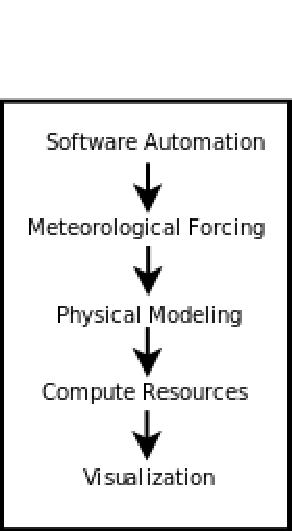
\includegraphics[width=19pc,angle=0]{closed_system.pdf}\\
  \caption{Enter the caption for your figure here.  Repeat as
  necessary for each of your figures.}\label{f1}
\end{figure}

%    D I S T R I B U T E D   C H A I N
\begin{figure}[t]
  \noindent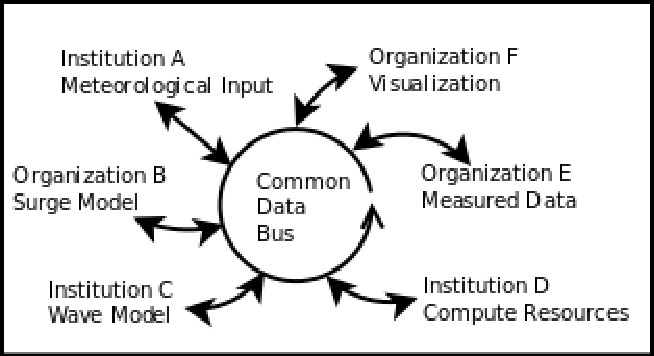
\includegraphics[width=19pc,angle=0]{distributed_chain.pdf}\\
  \caption{Enter the caption for your figure here.  Repeat as
  necessary for each of your figures.}\label{f1}
\end{figure}

%    A S G S   O V E R V I E W   F L O W C H A R T
\begin{figure}[t]
  \noindent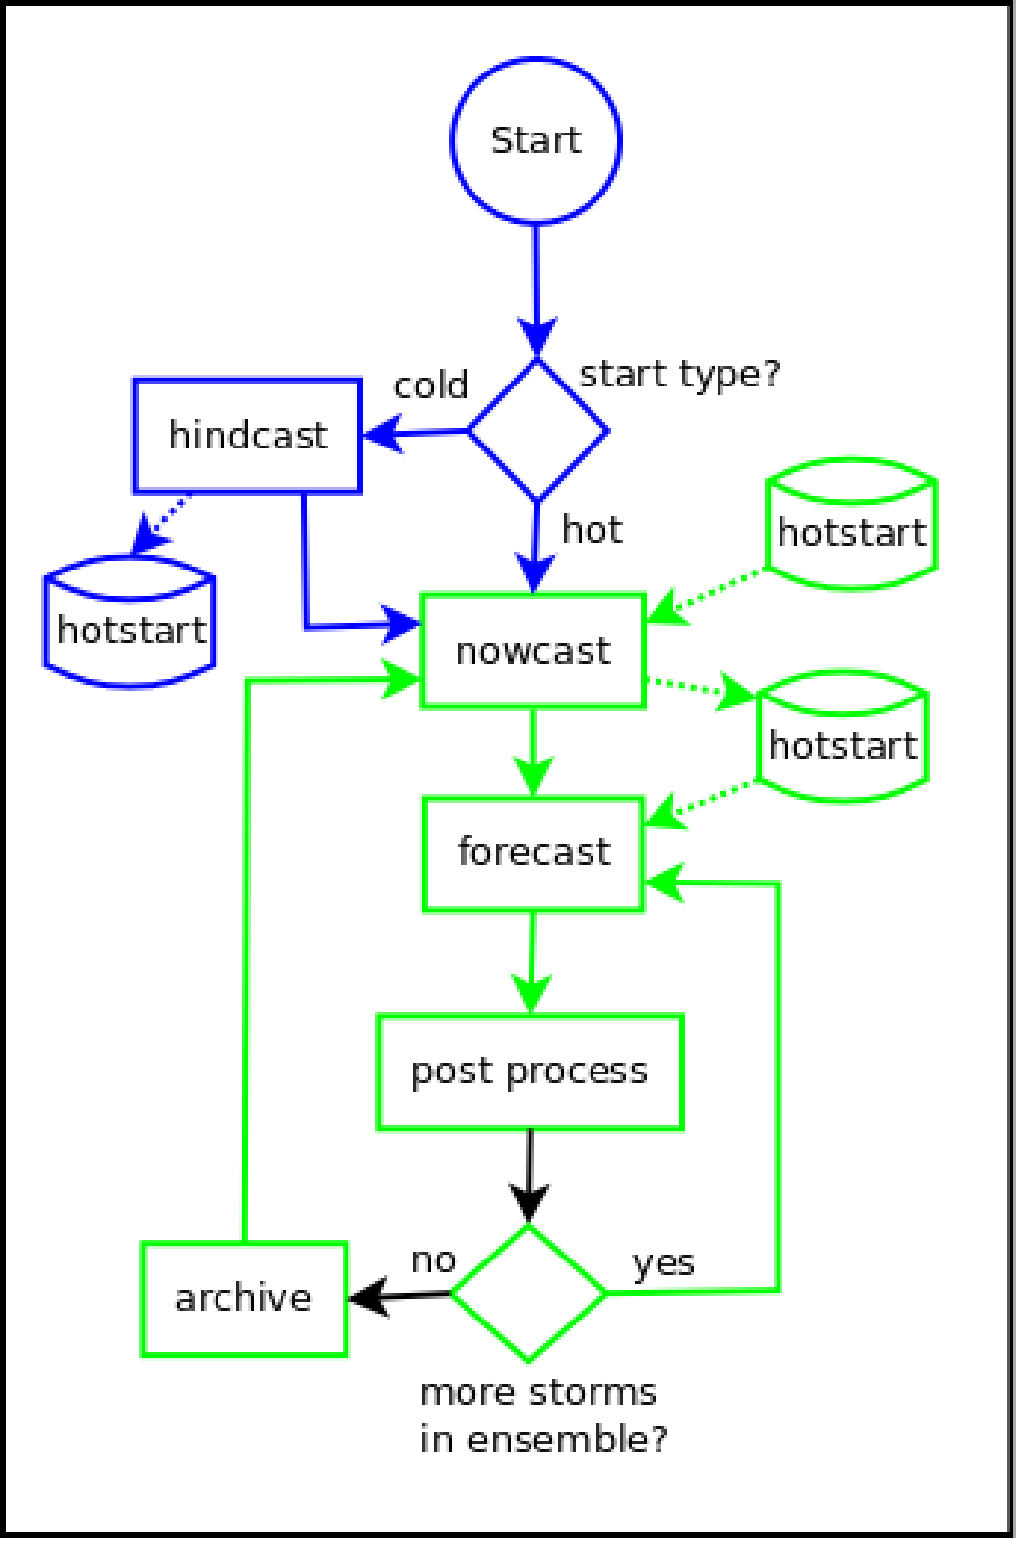
\includegraphics[width=19pc,angle=0]{asgs_overview_color.pdf}\\
  \caption{Enter the caption for your figure here.  Repeat as
  necessary for each of your figures.}\label{f1}
\end{figure}

%    A S G S   S T R U C T U R E   D I A G R A M 
\begin{figure}[t]
  \noindent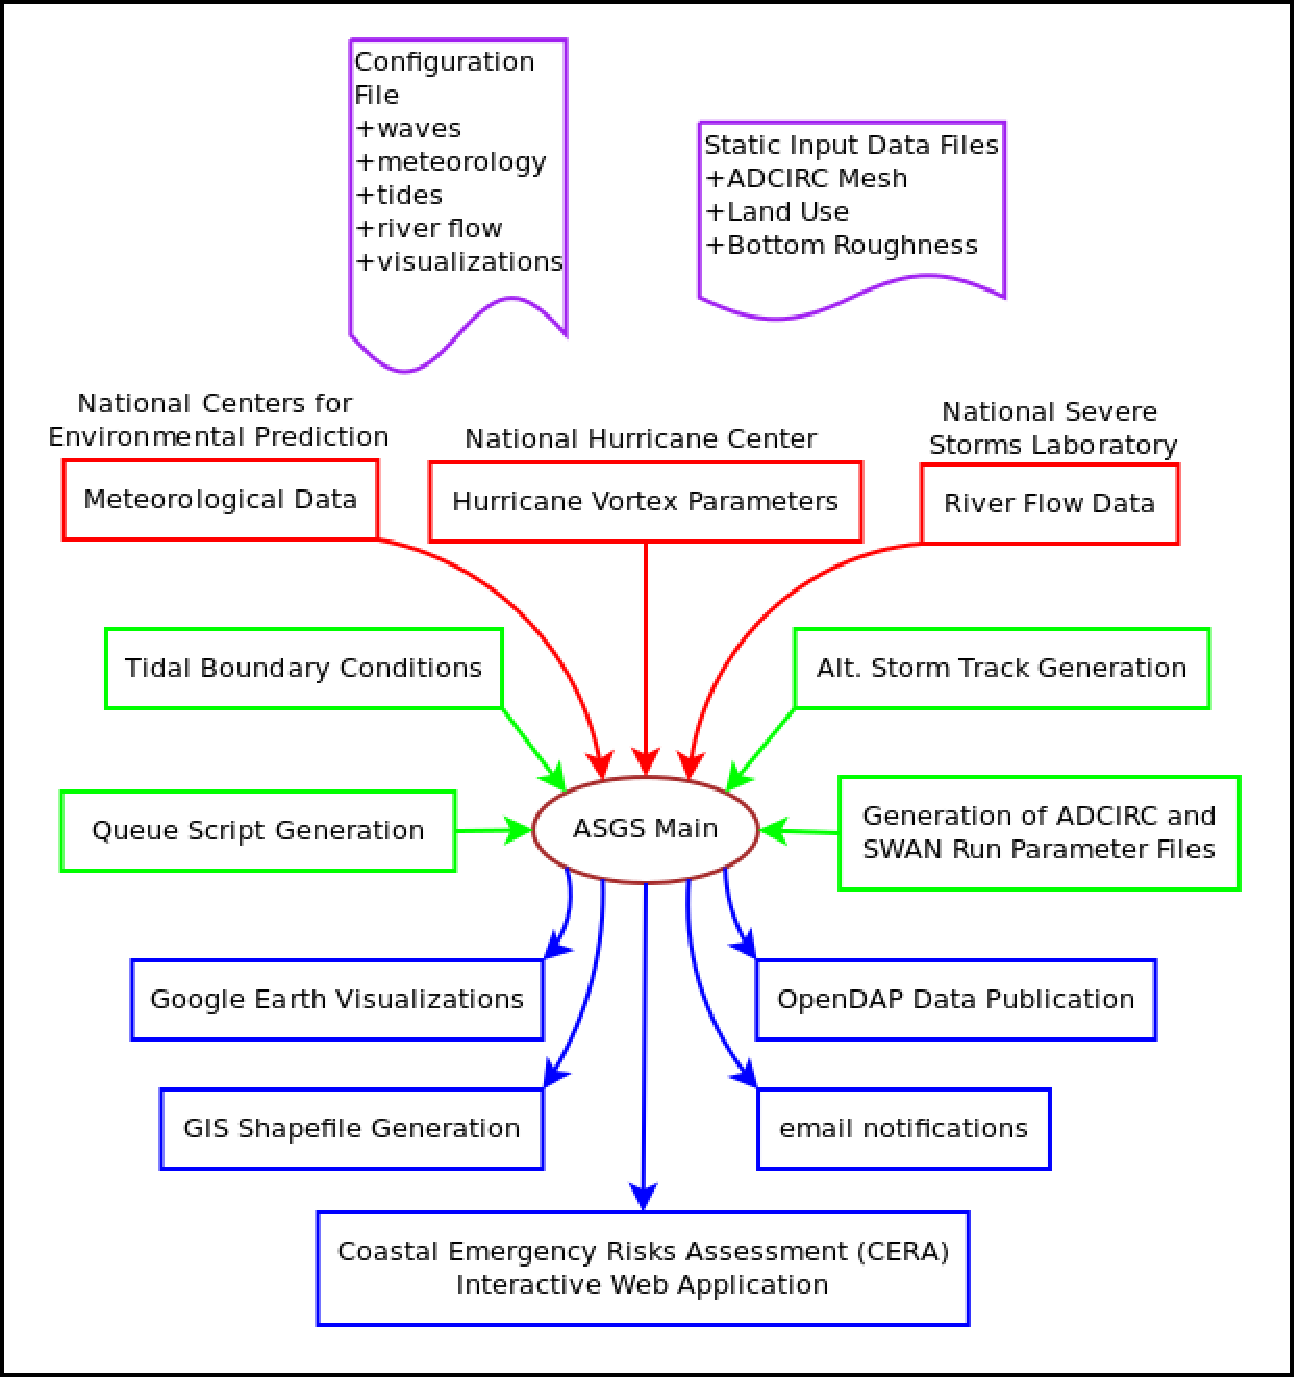
\includegraphics[width=19pc,angle=0]{asgs_structure_color.pdf}\\
  \caption{Enter the caption for your figure here.  Repeat as
  necessary for each of your figures.}\label{f2}
\end{figure}

%    N C   M E S H 
\begin{figure}[t]
  \noindent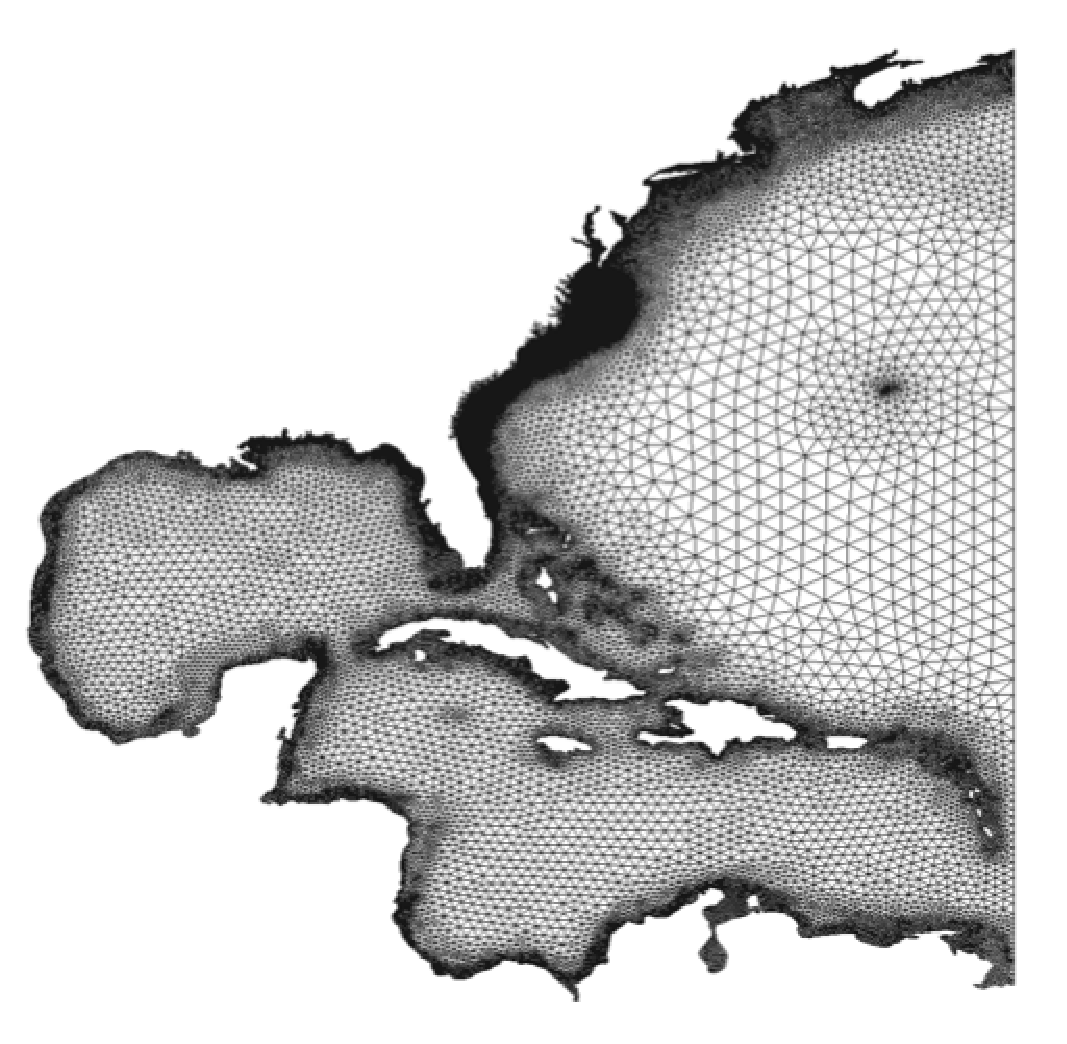
\includegraphics[width=19pc,angle=0]{ncv6b_mesh.pdf}\\
  \caption{Enter the caption for your figure here.  Repeat as
  necessary for each of your figures.}\label{f3}
\end{figure}

%    N C   B A T H Y
\begin{figure}[t]
  \noindent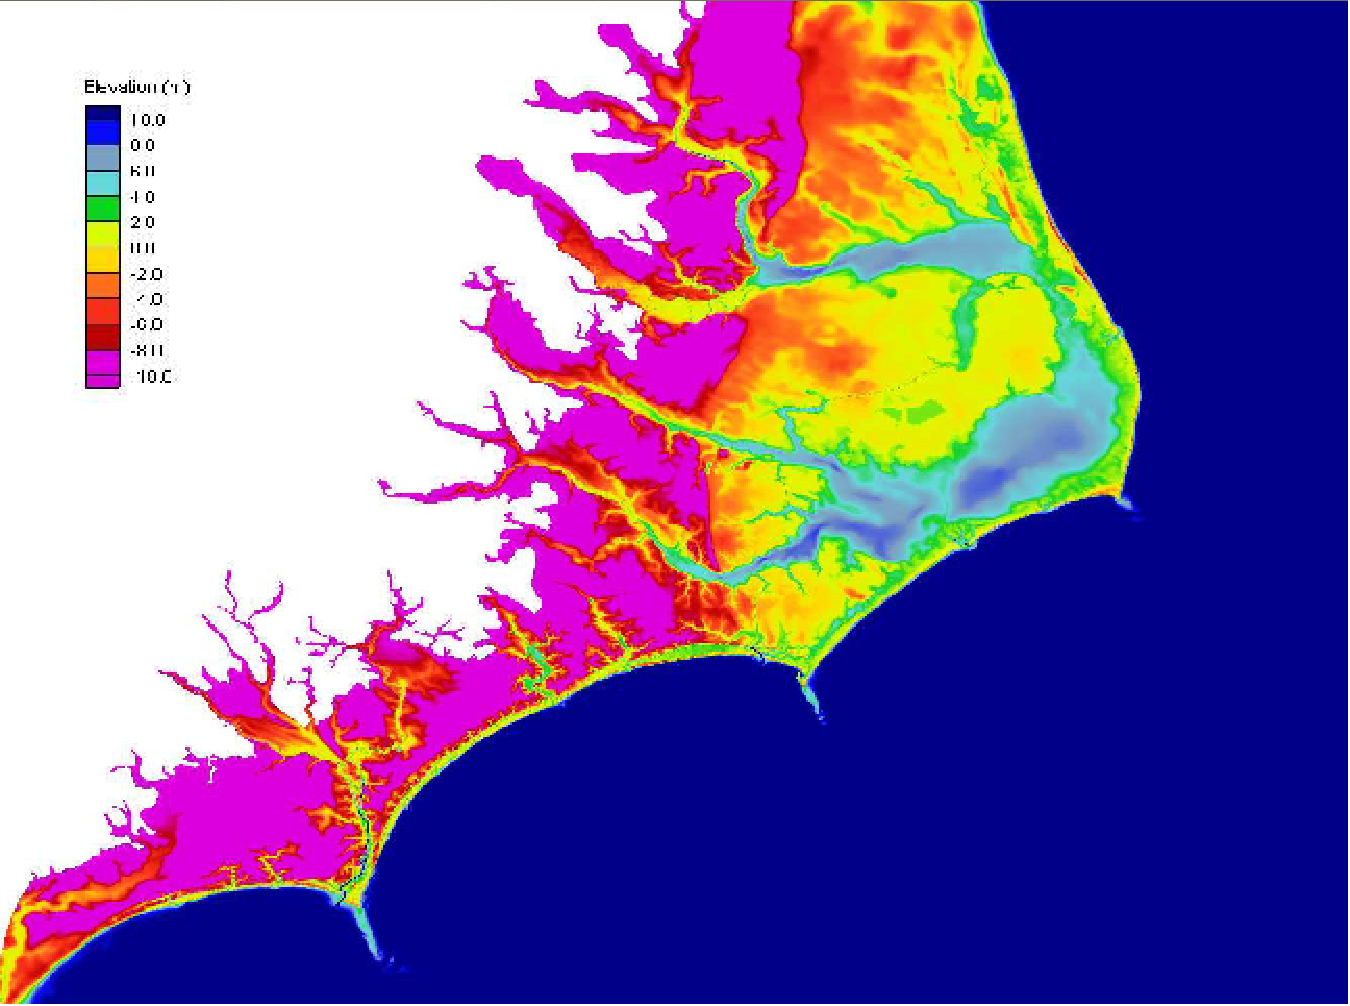
\includegraphics[width=19pc,angle=0]{ncv6b_bathy.pdf}\\
  \caption{Enter the caption for your figure here.  Repeat as
  necessary for each of your figures.}\label{f4}
\end{figure}

%    N C   L A N D C O V E R
\begin{figure}[t]
  \noindent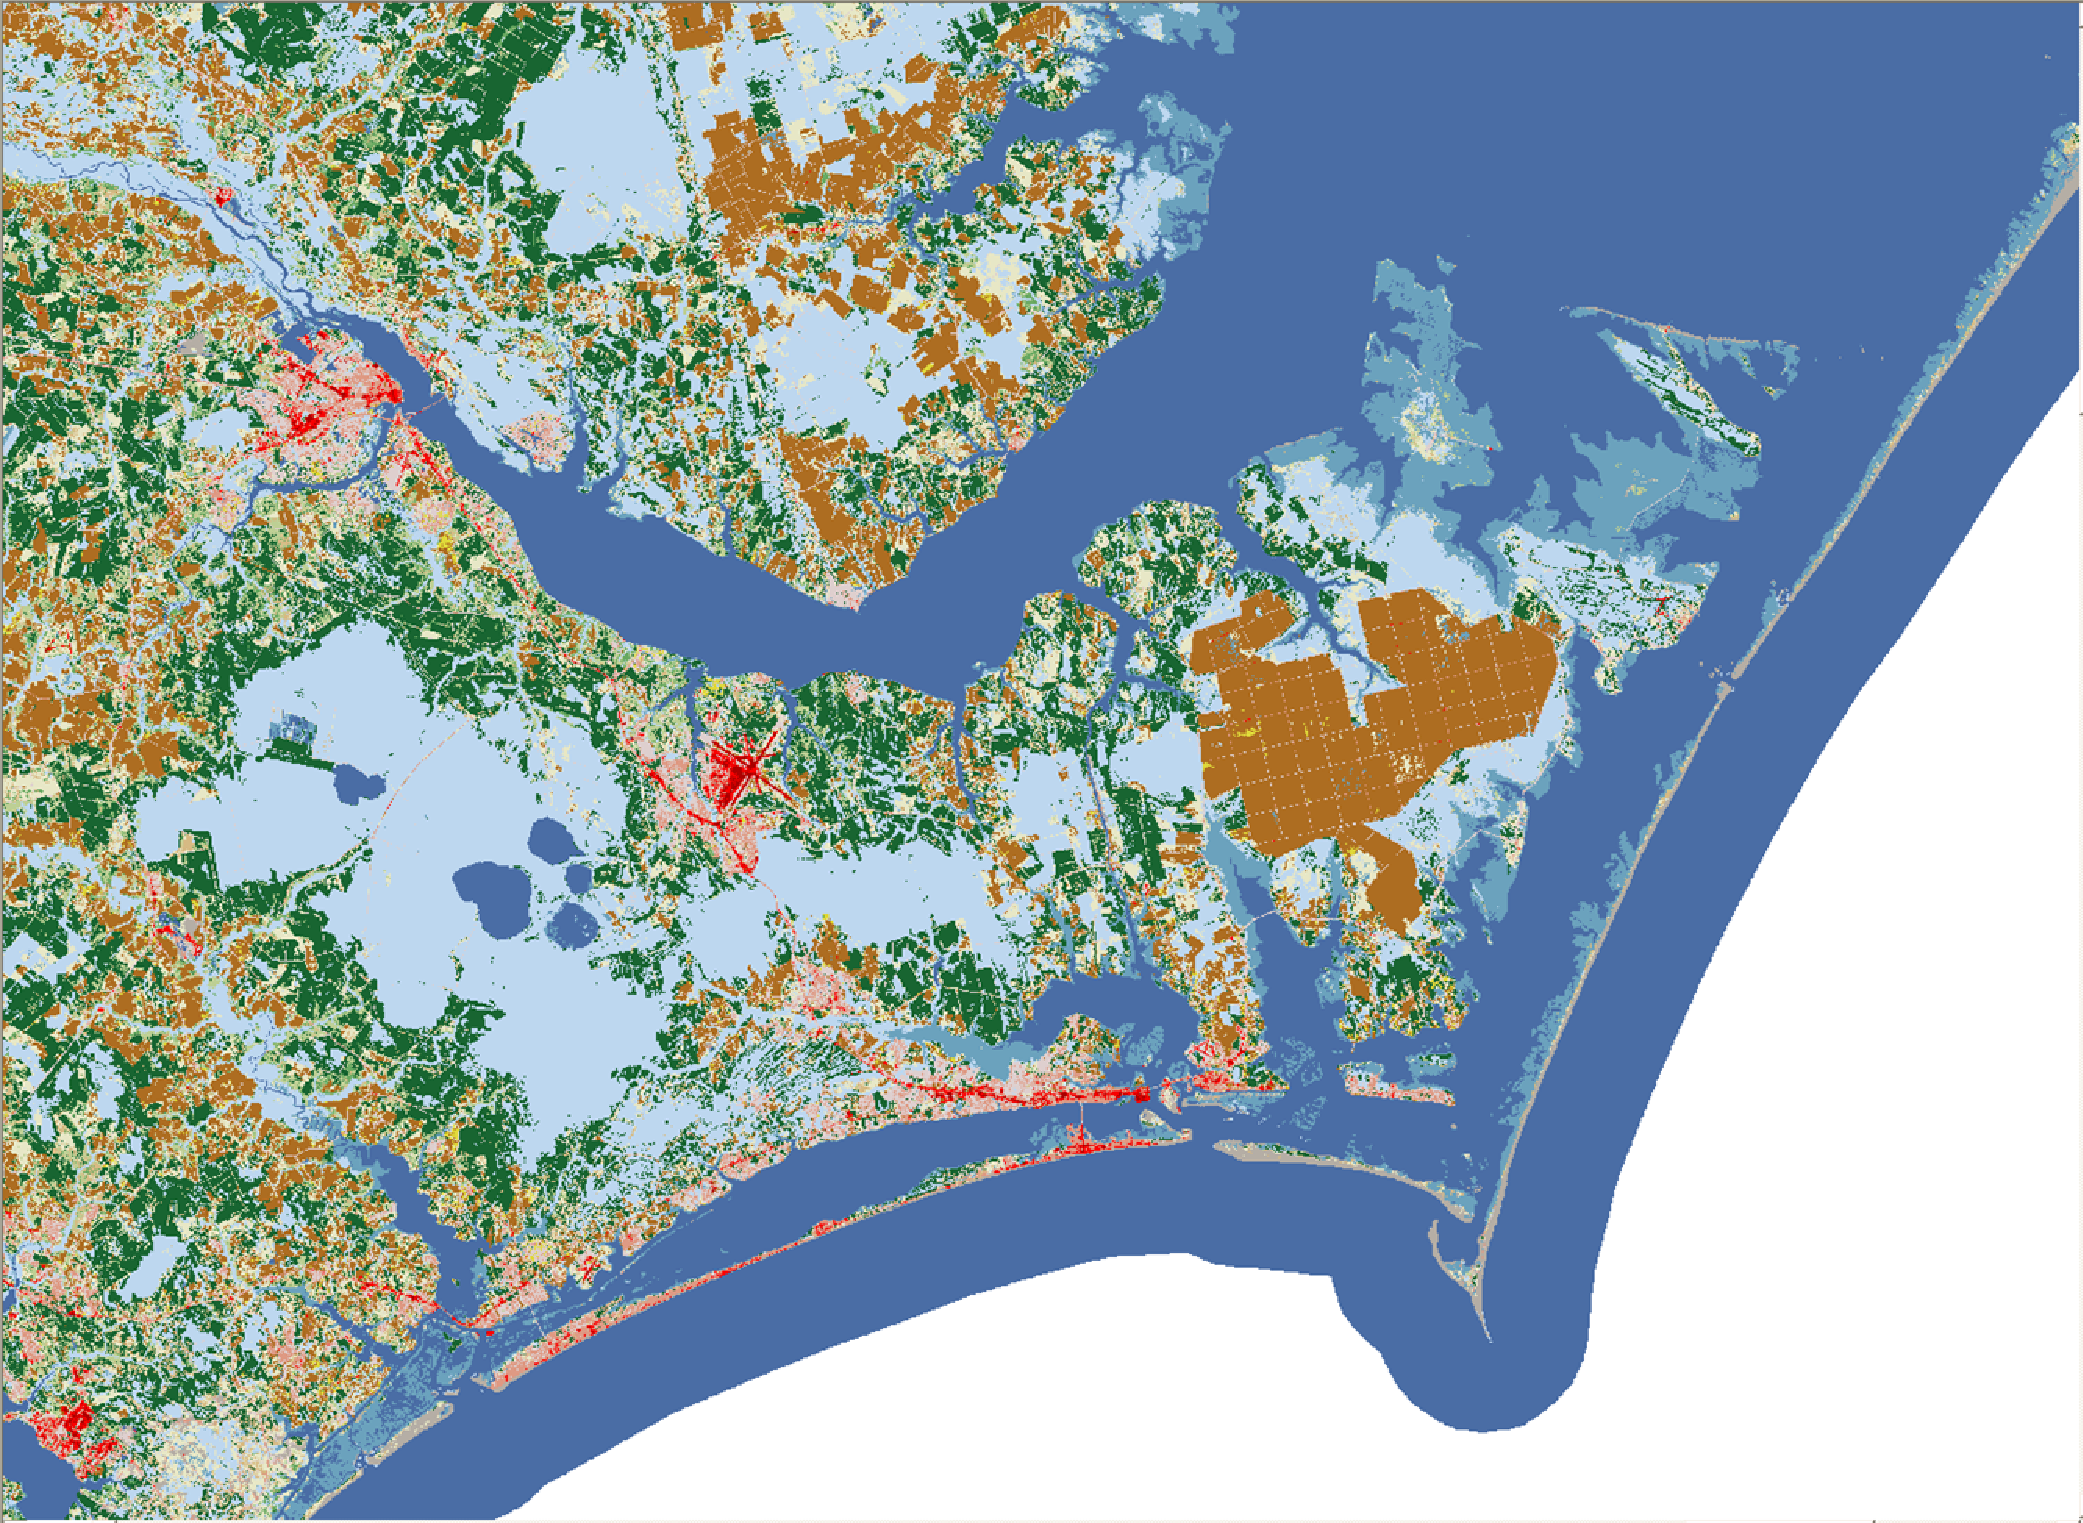
\includegraphics[width=19pc,angle=0]{nc_landcover.pdf}\\
  \caption{Enter the caption for your figure here.  Repeat as
  necessary for each of your figures.}\label{f5}
\end{figure}

%   S T O R M   P A R A M E T E R   V A R I A T I O N S
\begin{figure}[t]
  \noindent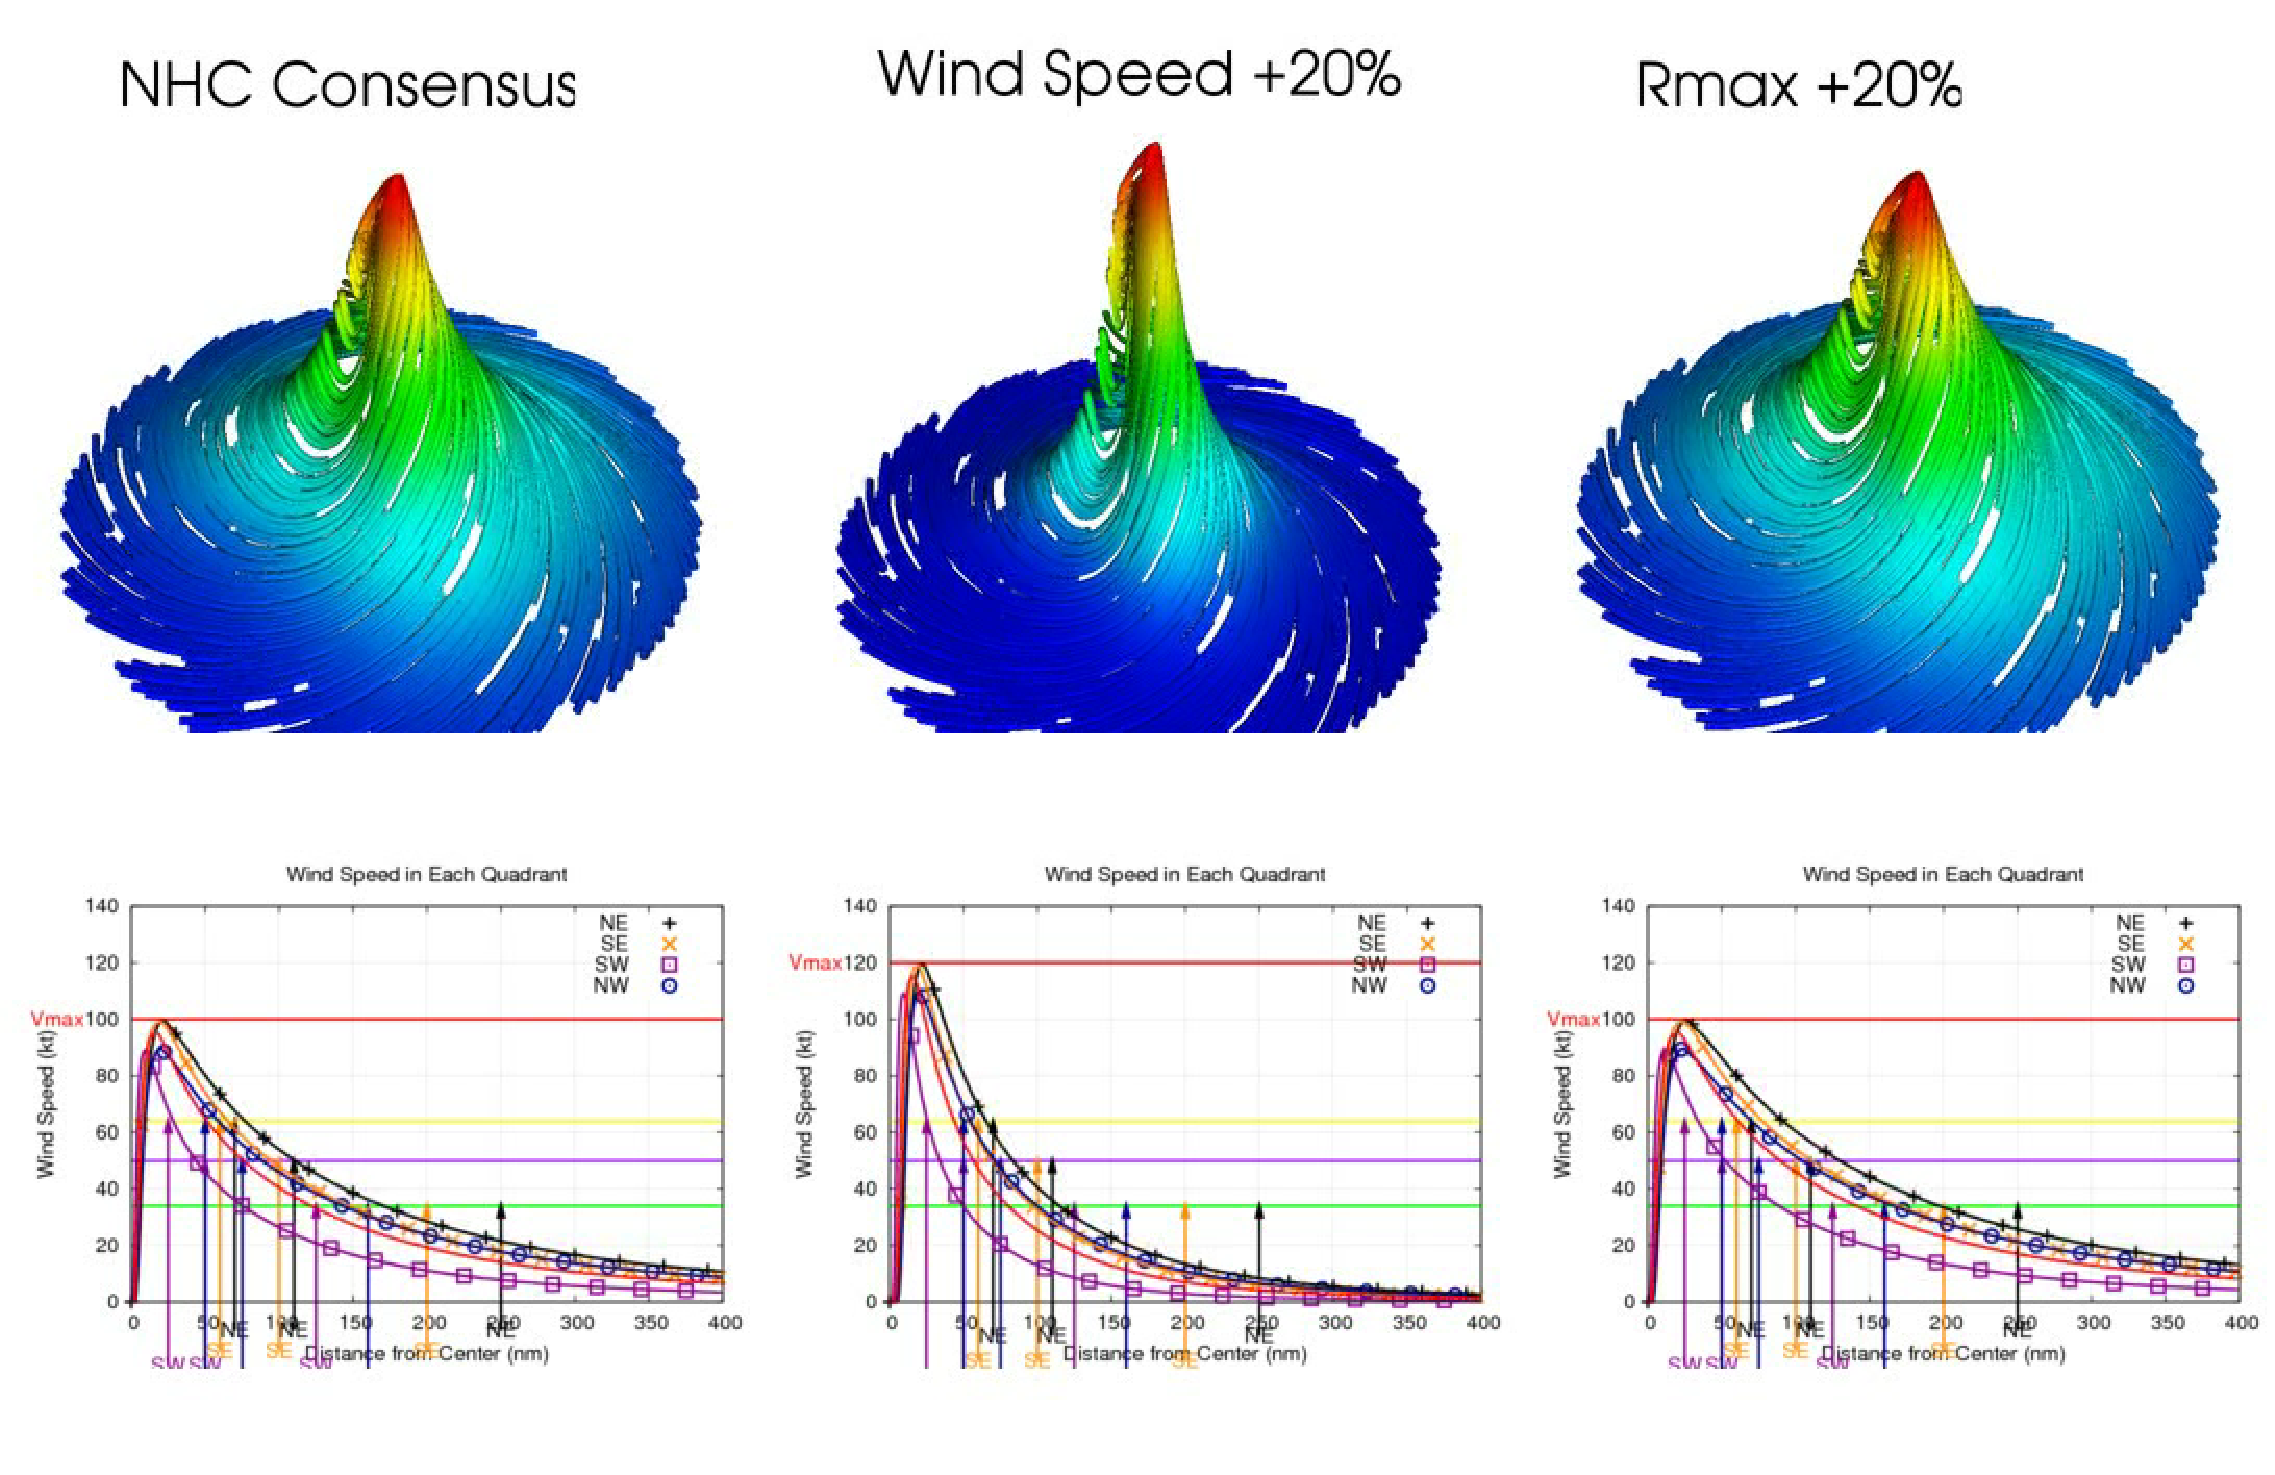
\includegraphics[width=40pc,angle=0]{variations.pdf}\\
  \caption{Enter the caption for your figure here.  Repeat as
  necessary for each of your figures.}\label{f6}
\end{figure}




%%%%%%%%%%%%%%%%%%%%%%%%%%%%%%%%%%%%%%%%%%%%%%%%%%%%%%%%%%%%%%%%%%%%%
% TABLES
%%%%%%%%%%%%%%%%%%%%%%%%%%%%%%%%%%%%%%%%%%%%%%%%%%%%%%%%%%%%%%%%%%%%%
%\begin{table}[t]
%\caption{This is a sample table caption and table layout.  Enter as many tables %as necessary at the end of your manuscript. Table from Lorenz (1963).}\label{t1}%
%\begin{center}
%\begin{tabular}{ccccrrcrc}
%\hline\hline
%$N$ & $X$ & $Y$ & $Z$\\
%\hline
% 0000 & 0000 & 0010 & 0000 \\
% 0005 & 0004 & 0012 & 0000 \\
% 0010 & 0009 & 0020 & 0000 \\
% 0015 & 0016 & 0036 & 0002 \\
% 0020 & 0030 & 0066 & 0007 \\
% 0025 & 0054 & 0115 & 0024 \\
%\hline
%\end{tabular}
%\end{center}
%\end{table}
%
\end{document}
